\chapter{The Money Order Office}
	 

\begin{marginfigure}
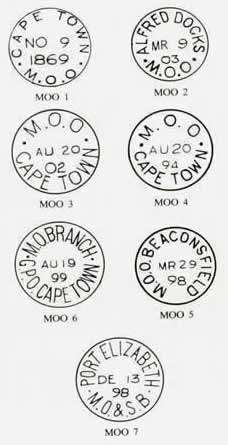
\includegraphics[width=.98\textwidth]{../cape-of-good-hope/moneyorderbranch/MOO-Stamps.jpg}
\caption{Datestamps used in the Money Order Office.}
\end{marginfigure}


 

The post office advised the public as early as 1828 that, owing to 
the great distances the mail was conveyed, it would not accept 
responsibility for money sent by mail being lost or stolen in transit.

When money was to be transmitted, the postmaster wrote "Money Letter" 
on the outside of the cover. A separate bag was provided for money 
letters and the driver of the postcart was told of its contents.

The public was advised that, as a precautionary measure, those who 
found it absolutely necessary to transmit money by mail should cut 
the notes in half diagonally, retaining one half until confirmation 
of the safe arrival of the other had been received. Special 
arrangements were made between the banks and the post office to 
recognise notes treated in this manner, subject to satisfactory 
explanation in the event of a loss.

Money order business was instituted at the post office on 1 March 1846 
and initially the G.P.O. at Cape Town made use of the Circular 
Date Stamp of 1853 (CDS 1) to date the orders. (4) A datestamp 
for the Money Order Office (MOO 1) was brought into use in about 1869. 
A circle with a diameter of 24,5 to 25 mm reads "Cape Town" at the 
top and has the letters M.O.O. for Money Order Office below. 
The day, month and year are centred in the circle in two lines. 
(See example on a Money Order Advice from Aliwal North).
 

Money order facilities were gradually extended to all the main 
post offices in the colony and some were issued with special 
circular datestamps (MOO 2). Postmasters who had not been 
furnished with special stamps used the ordinary office datestamps 
to date money orders. Money Order datestamps were also used by some
postmasters to deface stamps on letters and to stamp telegrams.


\ph[width = .70\textwidth]{../cape-of-good-hope/moneyorderbranch/Money-Order-Advice.jpg}{
1873 Money Order Advice 
complete form (106 x 142 mm) printed in orange-brown ex Aliwal North (town oval) 
AU 29 1873 in amount of eight pounds payable to the Secretary Mutual 
Life Assurance Society from Powrie and Brother showing receiving date stamp 
of Cape Town M.O.O. / SP 8 1873  (Goldblatt  MOO 1) at base 
endorsed to be returned.
}


The Cape Town Money Order Office used three different handstamps, 
which were brought into use about 1894. MOO 3 and MOO 4 are 
similar, both with the letters M.0.0. uppermost and the word 
Cape Town in the lower part of the circle. The diameter and the 
size of the lettering differ in the two types, that of MOO 3 
being 25 and 3,5 mm, respectively, whereas the diameter of MOO 4 
is 26 mm and the lettering 4,5 mm.

The third type (MOO 5) shows "M.O. Branch" at the top of the 
circle and "G.P.O. Cape Town" below. MOO 6 has the letters 
M.0.0. preceding the name of the town (in this instance, Beaconsfield). 
In 1898, Port Elizabeth received a datestamp of 25 mm diameter (MOO 7) 
which was in use for both the Money Order and Savings Bank branches, 
indicated by the abbreviation M.O. \& S.B. The Money Order Office 
at the General Post Office in Cape Town used a large and 
distinctive stamp (MOO 8), struck when the order was paid out 
on presentation. The design consists of double-lined inner and 
outer circles, with diameters of 30 and 45 mm respectively. 
The words "General Post Office" appear above, and "Cape Town" below, 
within the circles, and are separated by a star on either side. 
The word "Paid" framed by horizontal lines above and below, 
appears in the centre 3.

 
    